%%%%%%%%%%%%%%%%%%%%%%%%%%%%%%%%%%%%%%%%%%%%%%%%%%%%%%%%%%%%%%%%%%%%%%%
% Created on Mon Dec 6, 2023
% @author: Giselle Labrador Badia (@gisslab)


% Description:
%
% This shows reports on the DID exposure analysis.


%%%%%%%%%%%%%%%%%%%%%%%%%%%%%%%%%%%%%%%%%%%%%%%%%%%%%%%%%%%%%%%%%%%%%%%




\documentclass[11pt,a4paper]{article}


\usepackage[utf8]{inputenc}
\usepackage[spanish,english]{babel}
\usepackage{apacite}
\usepackage[round]{natbib}
\usepackage{hyperref}
\bibliographystyle{apacite}


\usepackage[margin = 1in, top=1.5cm,bottom=1.5cm]{geometry}% Margins
\setlength{\parindent}{2em}
\setlength{\parskip}{0.3em}
\usepackage{setspace} % Setting the spacing between lines
\usepackage{hyperref} % To create hyperlinks within the document
\spacing{1.15}

%images
\usepackage{graphicx}
% \usepackage{subcaption}
\usepackage{caption}
% subcaption was interfering with the figure count, fix below
\usepackage{subcaption, xparse}

% to read mid-rule
\usepackage{booktabs}

\usepackage[capposition=top]{floatrow}
\captionsetup[sub]{font=footnotesize,labelfont={bf,sf}}

\begin{document}

\title{Effects of QE on Ob Auctions \\ Dynamic DiD Exposure Analysis}

\maketitle

\section{FED purchases and investors}

\begin{table}[h]
    \centering
    \begin{tabular}{lr}
\toprule
                         Counterparty &  Amount (millions \$) \\
\midrule
             Morgan Stanley \& Co. LLC &        304942.000000 \\
    Credit Suisse AG, New York Branch &        250823.000000 \\
        Citigroup Global Markets Inc. &        147080.000000 \\
              Goldman Sachs \& Co. LLC &        135429.000000 \\
                BofA Securities, Inc. &        120978.000000 \\
                    J.P. Morgan Chase &        107276.000064 \\
               Wells Fargo Securities &         85703.000000 \\
                Barclays Capital Inc. &         75758.000000 \\
Nomura Securities International, Inc. &         72998.999872 \\
   Daiwa Capital Markets America Inc. &         46478.000000 \\
                          BNP-Paribas &         17412.000000 \\
            Mizuho Securities USA LLC &          9715.000000 \\
                        Jefferies LLC &          6345.000000 \\
\bottomrule
\end{tabular}

    \caption{Sold amount in period Jul 2019 to April 2021}\label{tab:descriptive}
    % \begin{minipage}{\textwidth}
    %     \footnotesize{\textit{Notes:}  } 
    %     \end{minipage}
\end{table}

There are 931 from  14873 observations in this period that have a missing counterparty (investor).

\pagebreak
\begin{figure}[h]
    \centering
    \begin{subfigure}[b]{0.65\textwidth}
        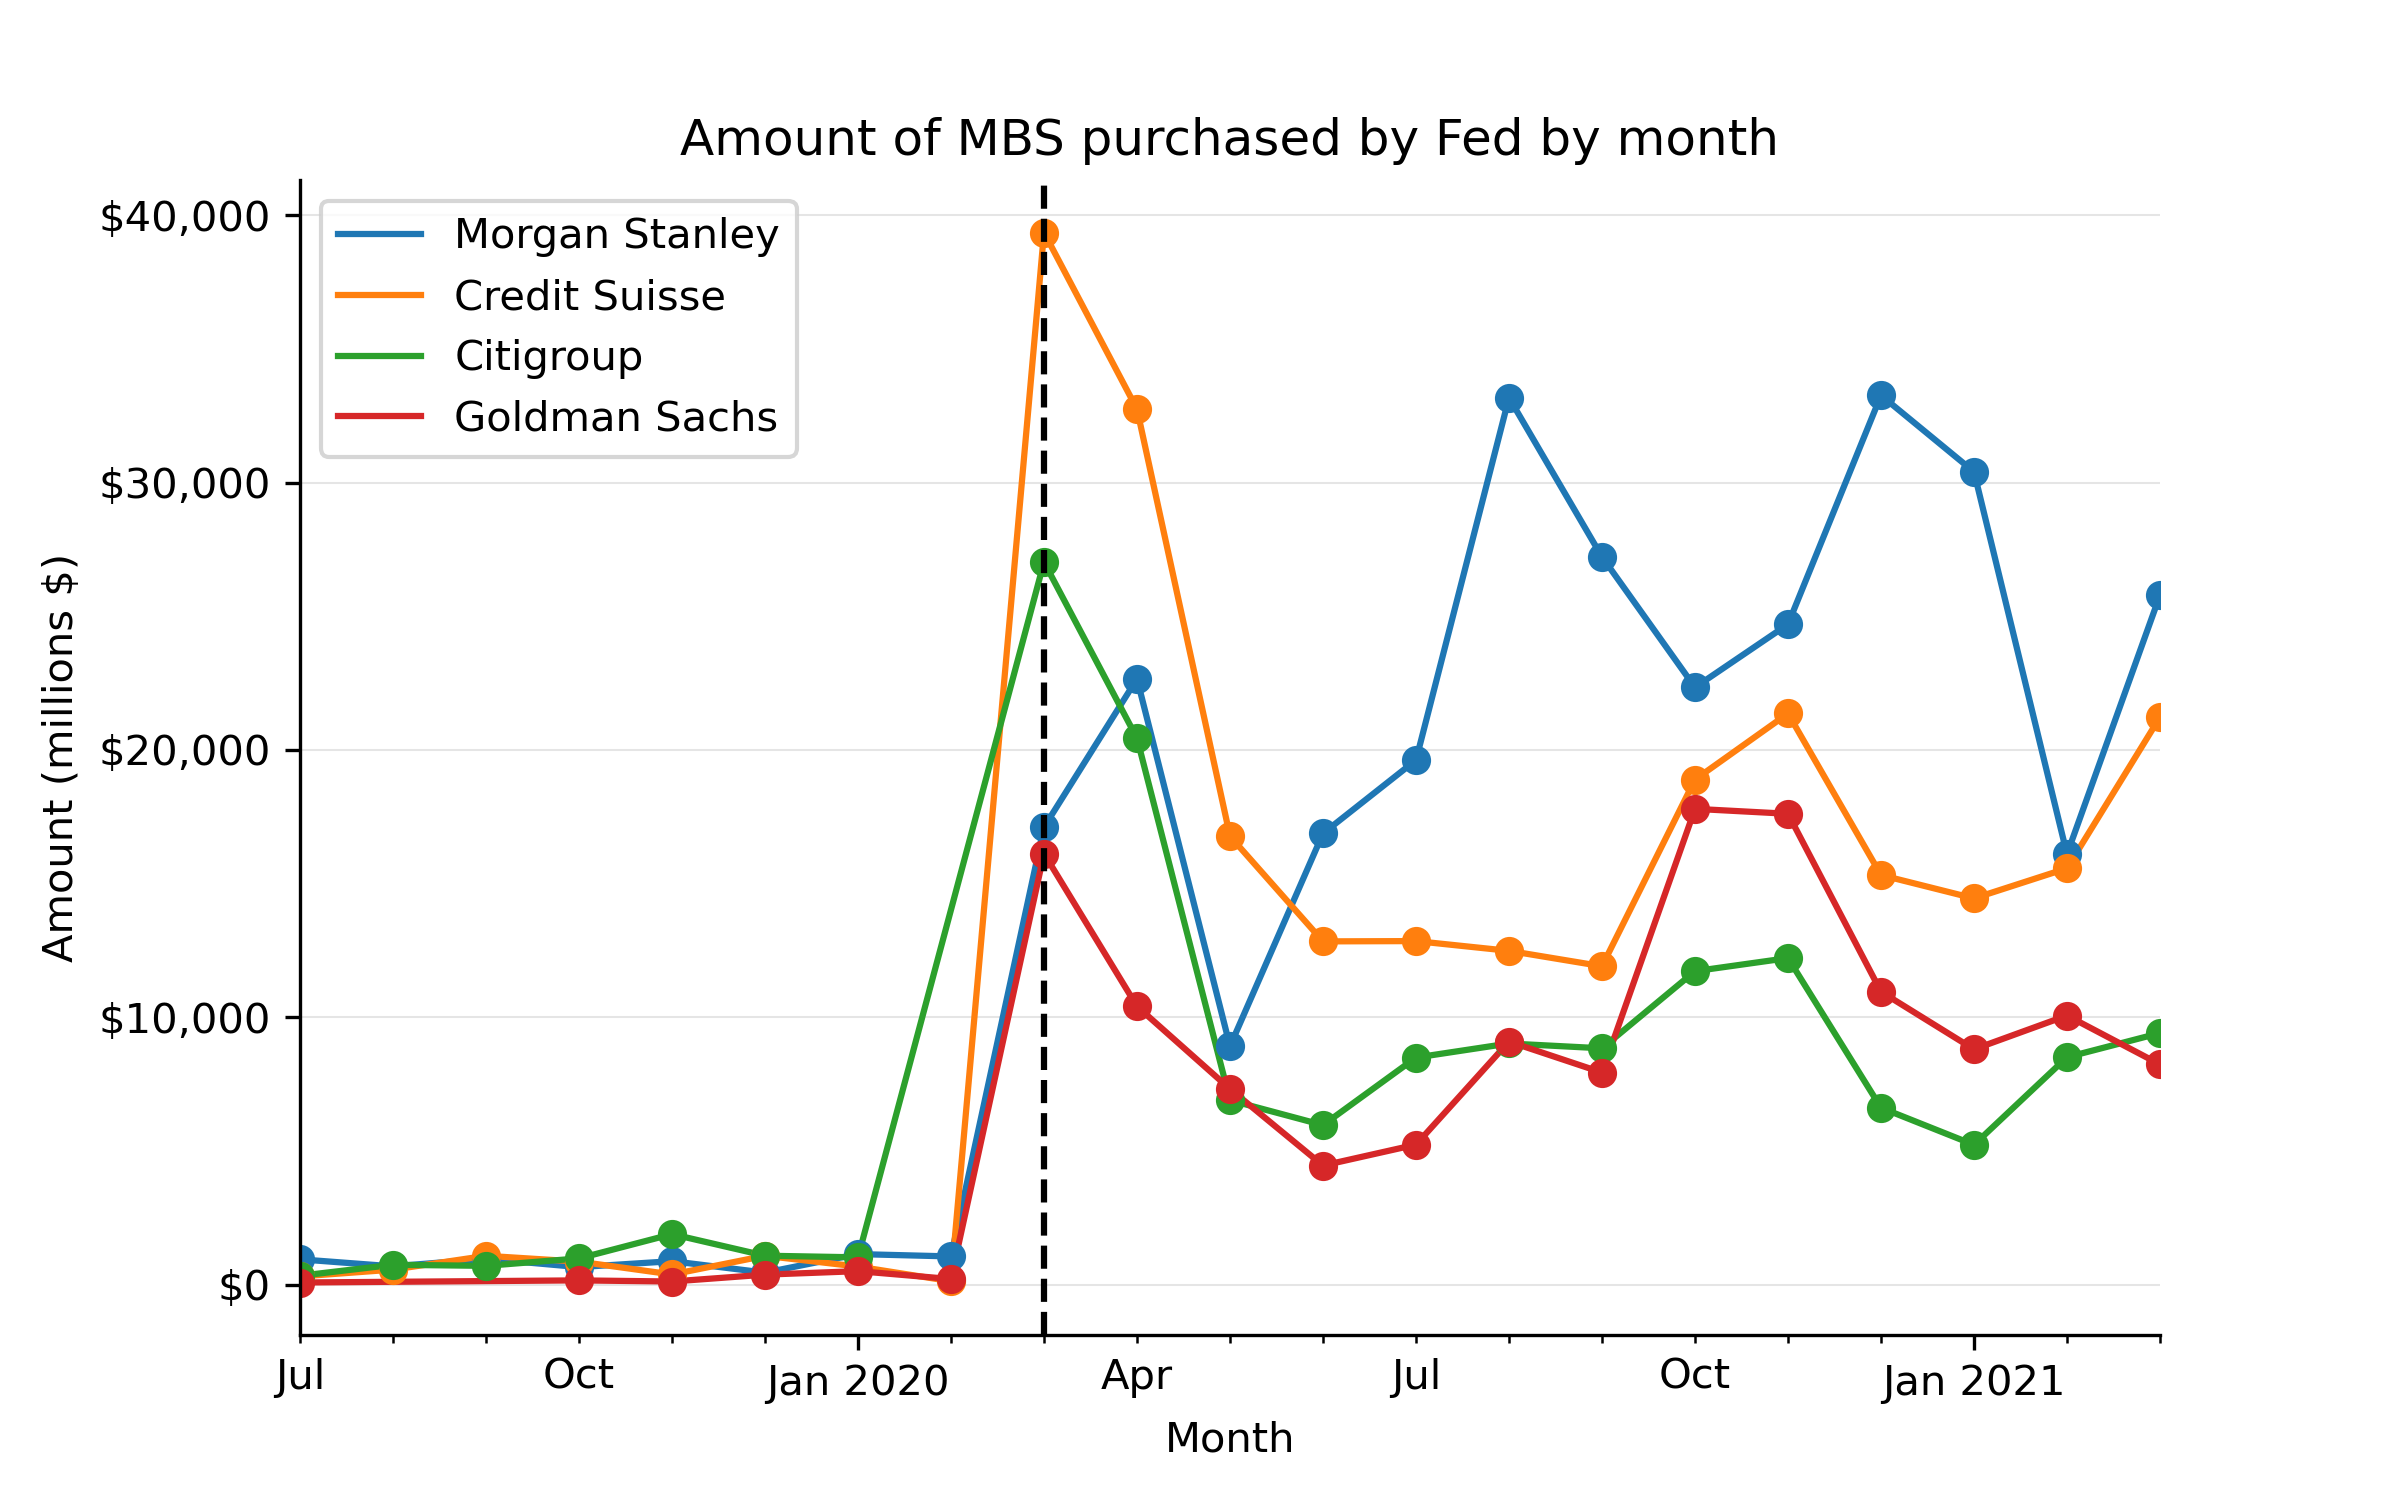
\includegraphics[width=0.98\textwidth]{../results/figures/fed_mbs_amount_by_month_example_larg4.png}
        \caption{Largest 4 investors that sold loans to the FED.}\label{fig:larg4}
       \end{subfigure}
       \begin{subfigure}[b]{0.65\textwidth}
        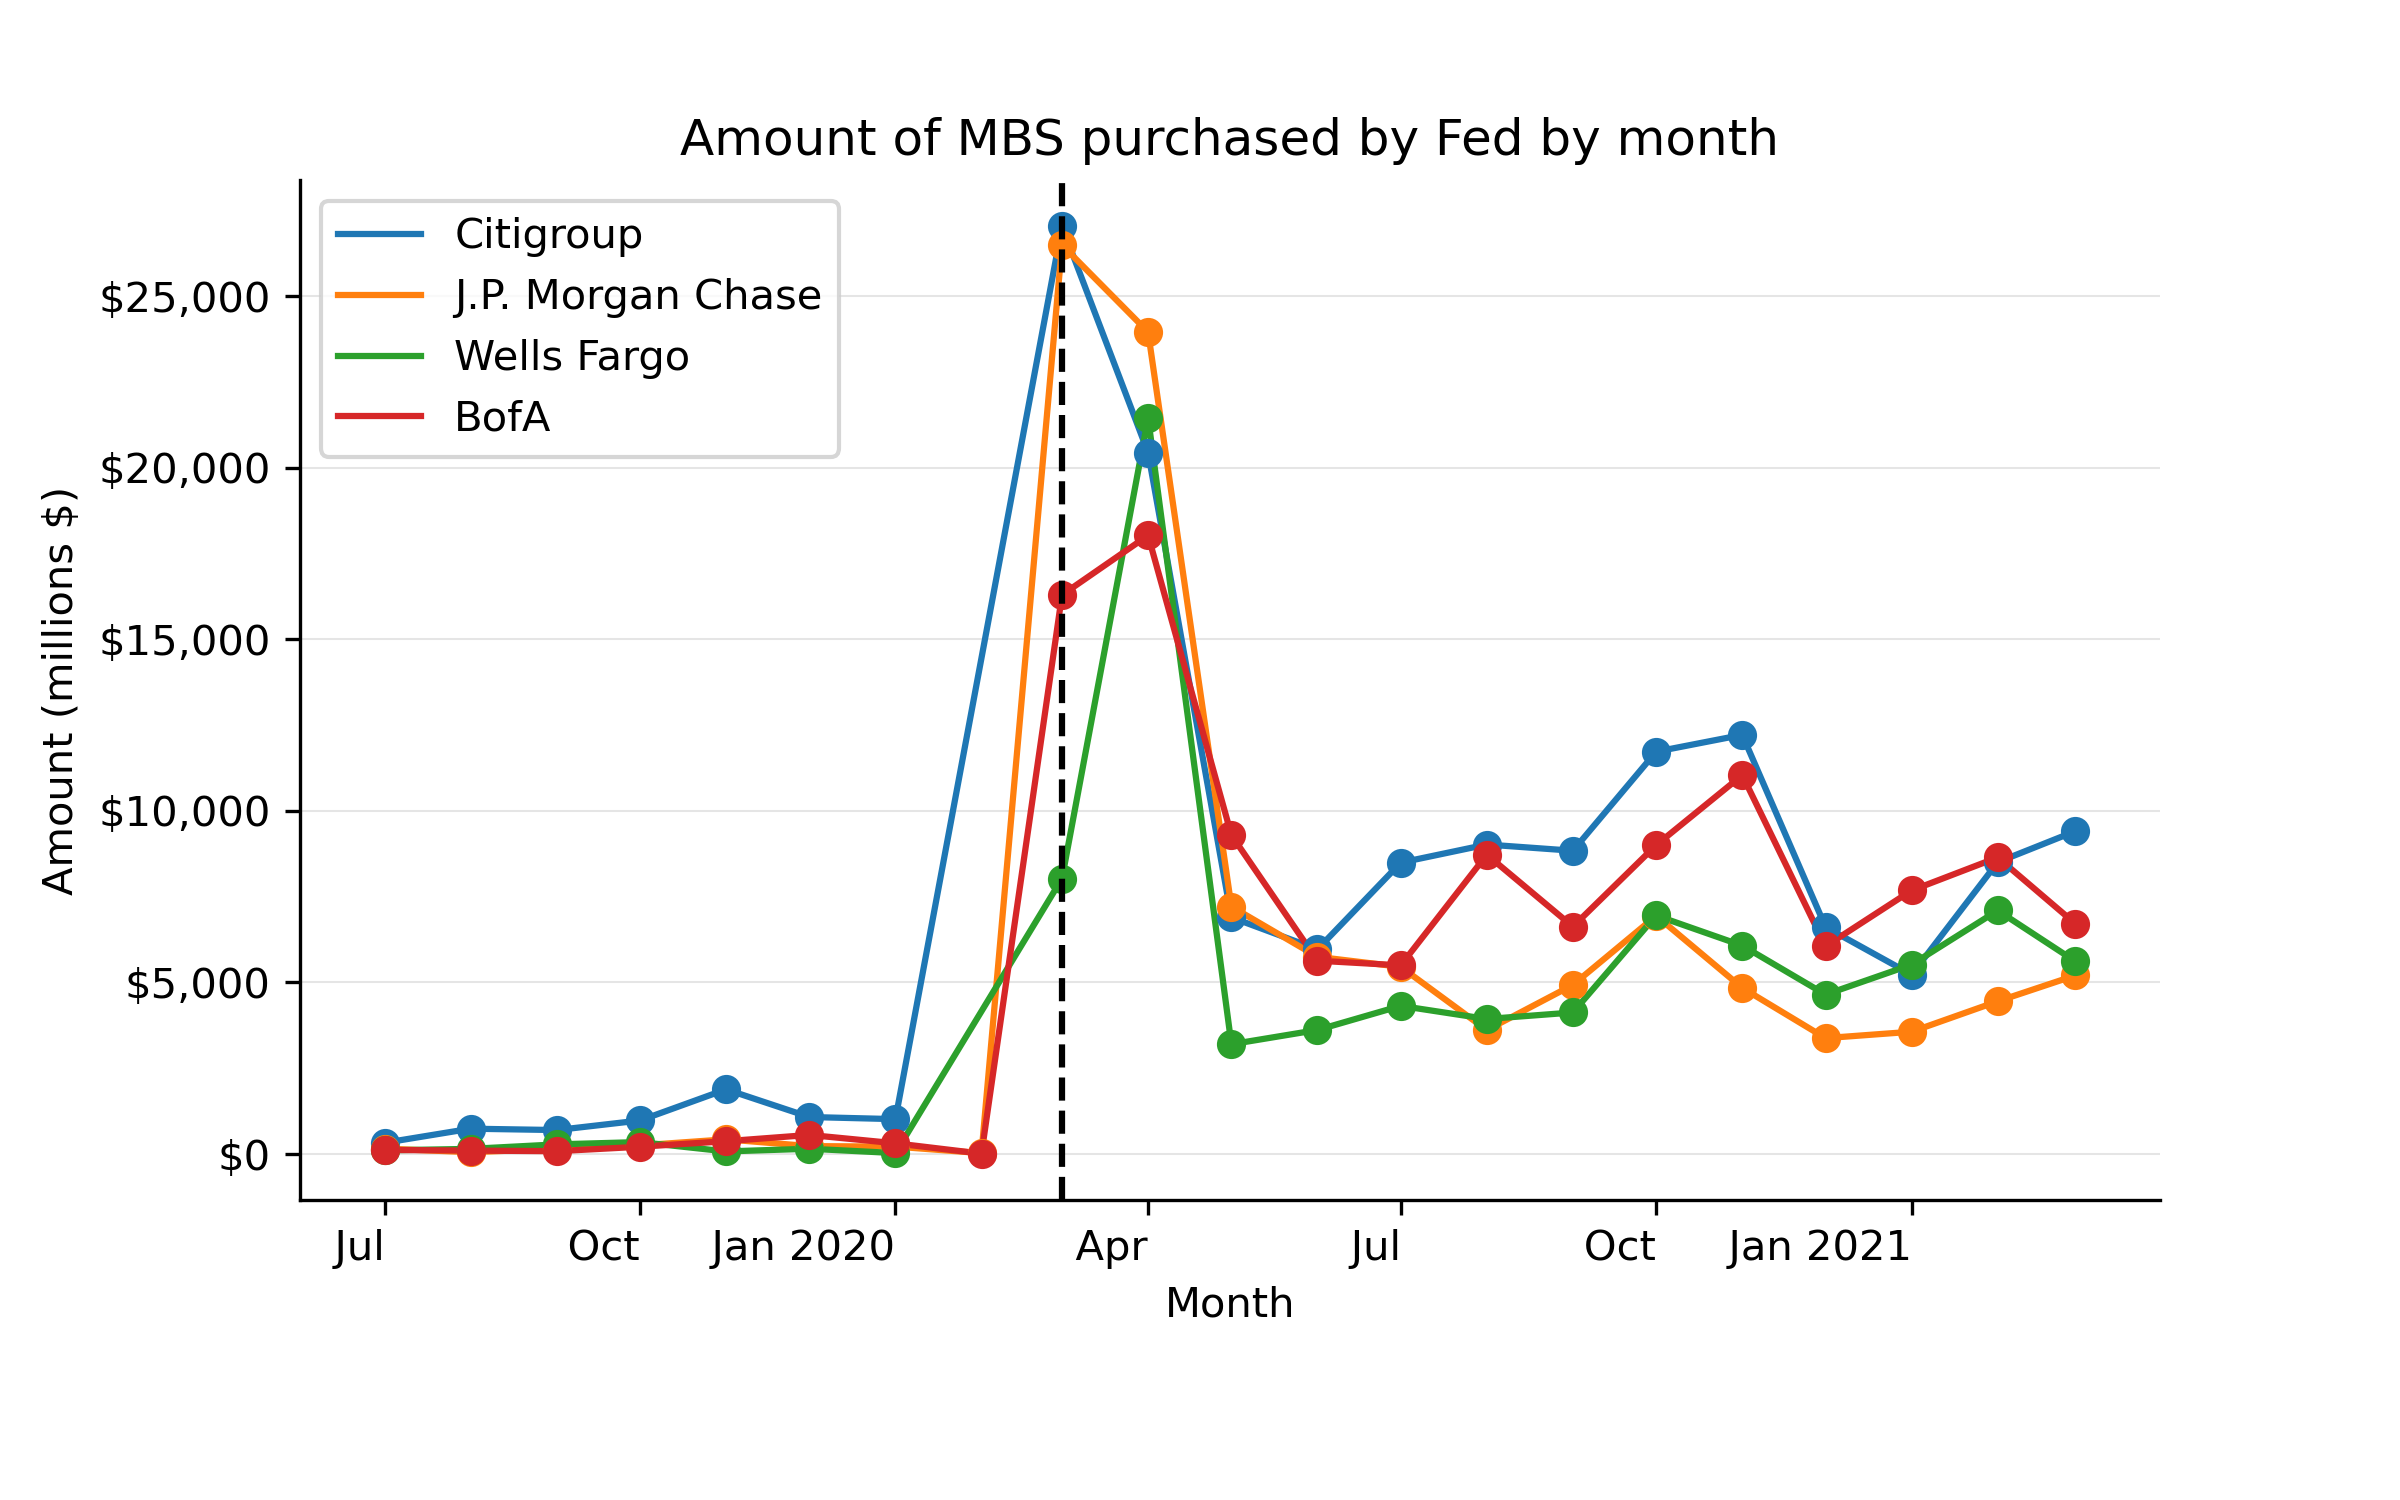
\includegraphics[width=0.999\textwidth]{../results/figures/fed_mbs_amount_by_month_example_retail.png}
        \caption{ Commercial banks } 
       \end{subfigure}
       \caption{FED MBS purchases by month.}\label{fig:fed_mbs_amount_by_month}
     \begin{minipage}{\textwidth}
        \footnotesize{\textit{Notes:} The figure shows a time series of FED auction outcomes. The vertical line is March 1.  } 
        \end{minipage}
  \end{figure}


%   \begin{figure}[h]
%     \centering
%        \begin{subfigure}[b]{0.6\textwidth}
%         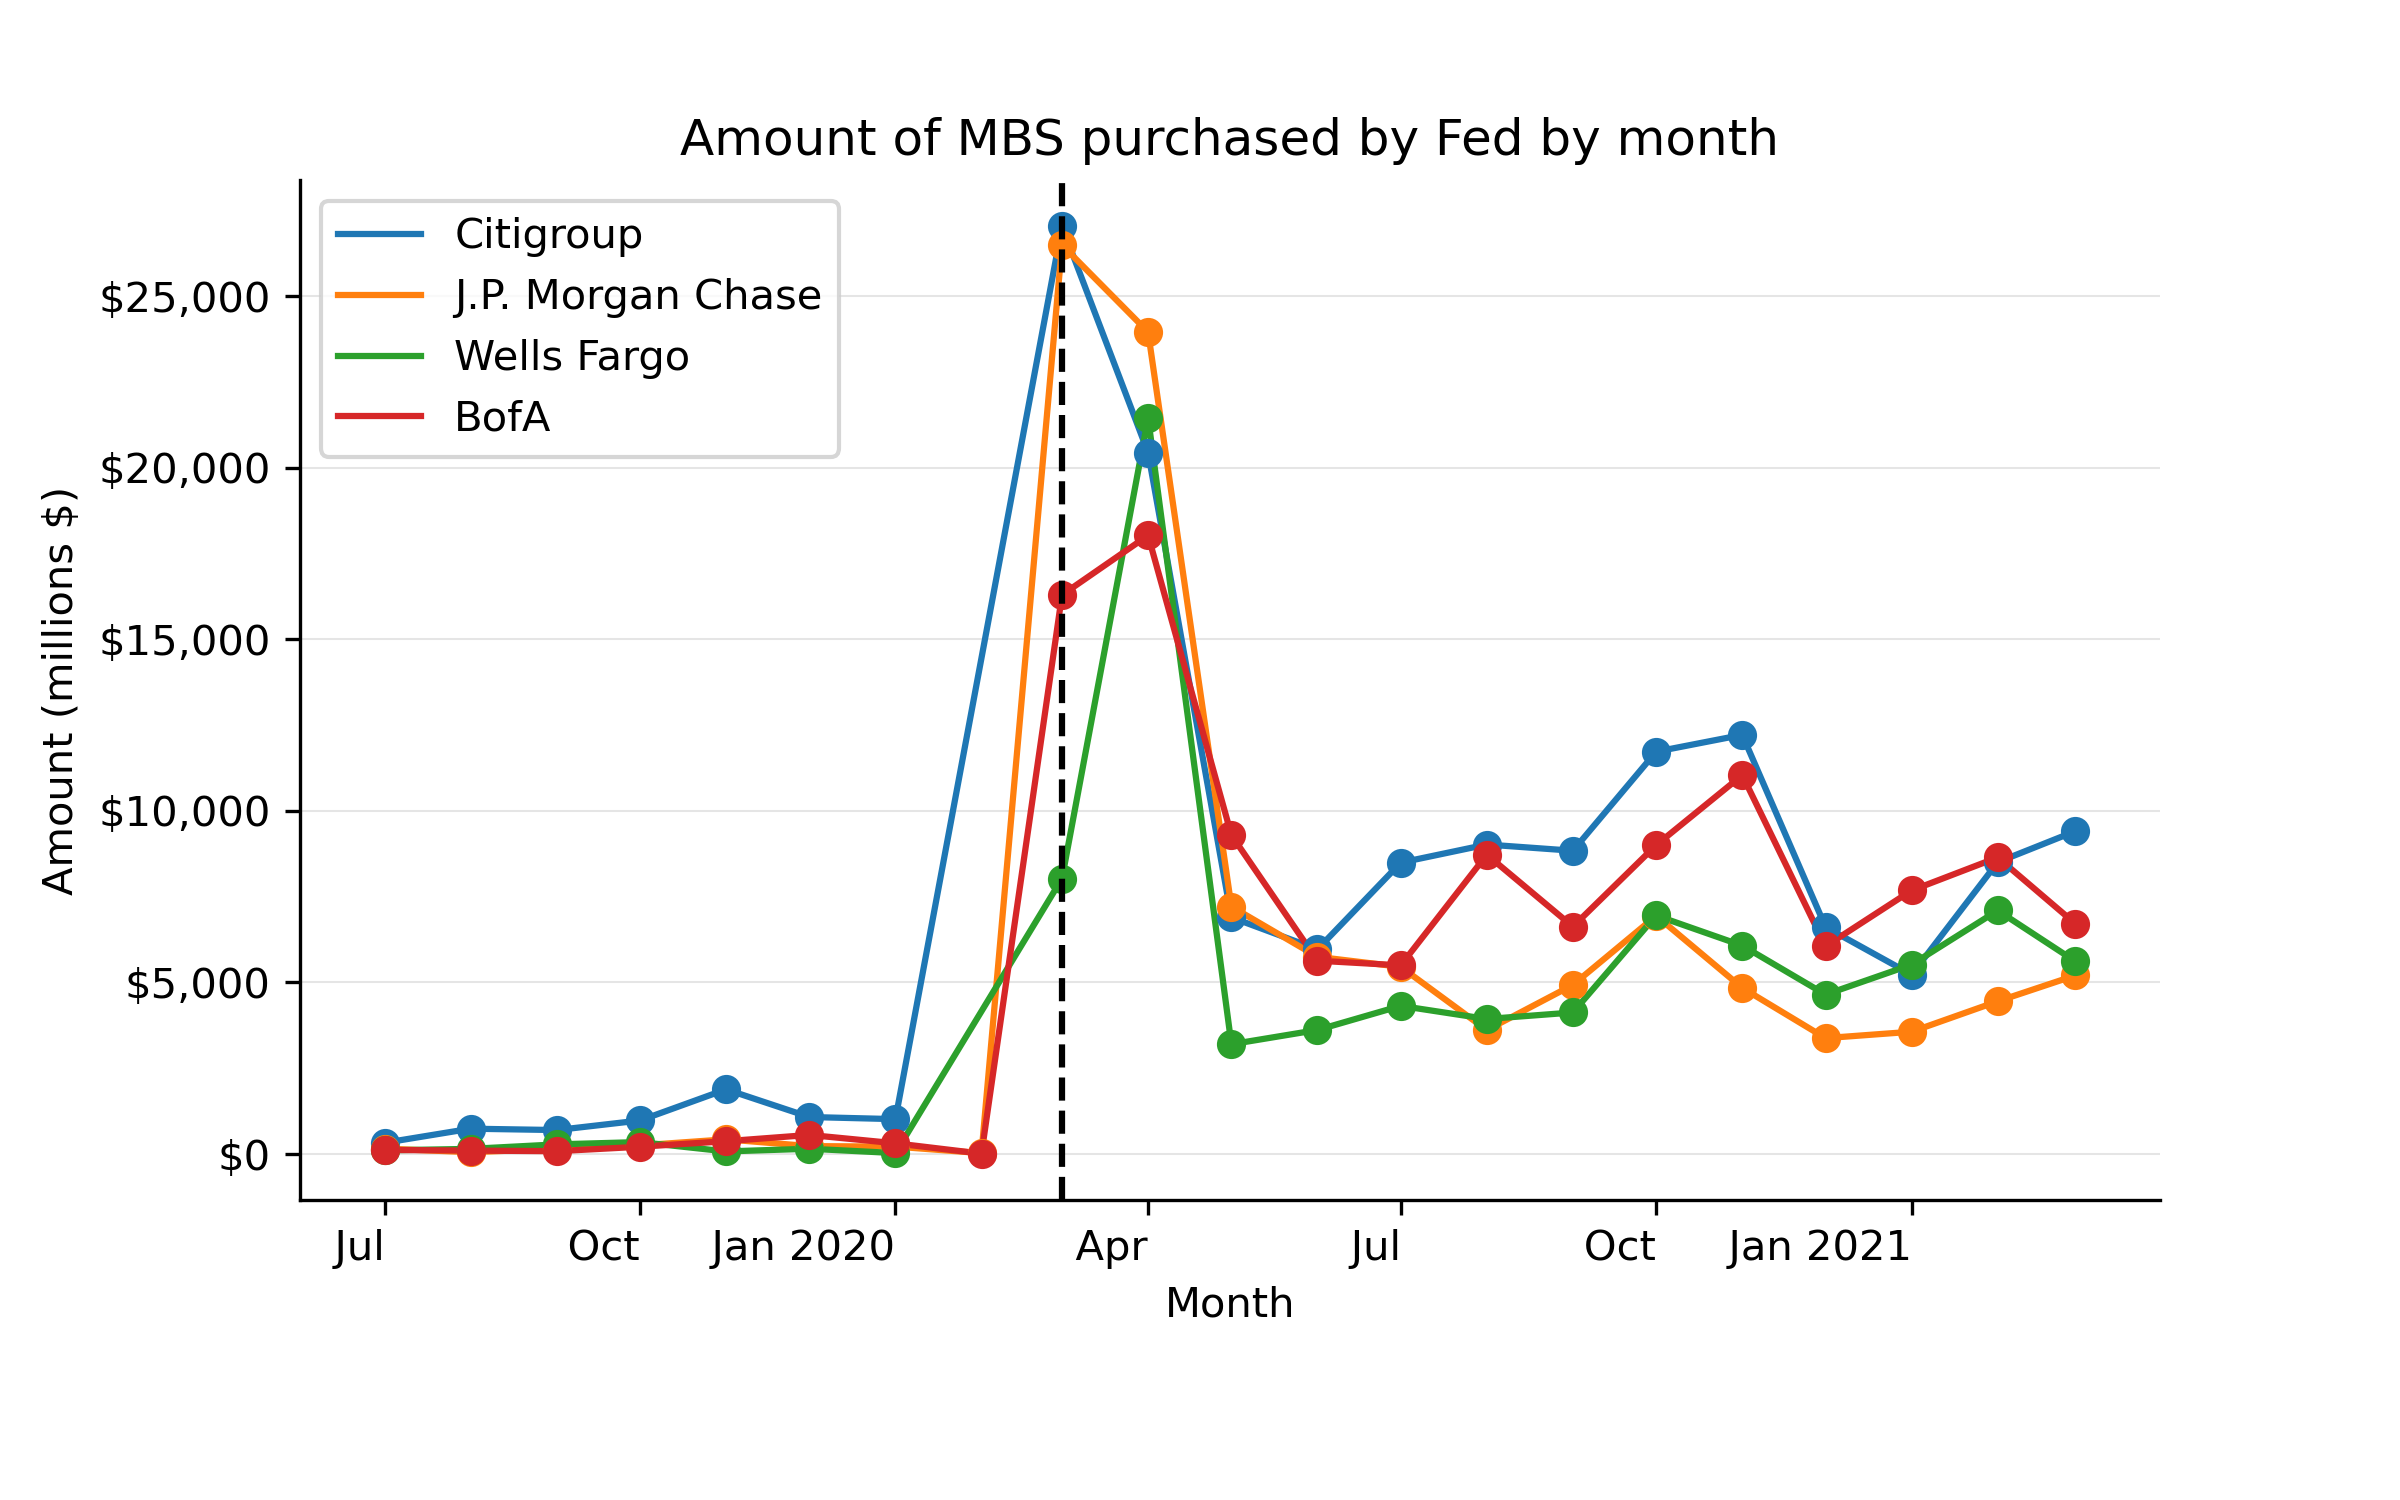
\includegraphics[width=0.999\textwidth]{../results/figures/fed_mbs_amount_by_month_example_retail.png}
%         \caption{ Bid difference between Freddie and Fannie.}
%        \end{subfigure}
%        \caption{OB auction  GSE response for coupon 2.5 } 
%      \begin{minipage}{\textwidth}
%         \footnotesize{\textit{Notes:} The figure shows a time series of FED auction outcomes. The vertical line is March 1.  } 
%         \end{minipage}
%   \end{figure}

\pagebreak

\section{Dynamic DiD Exposure Analysis}

The dynamic DiD analysis is based on the following equation:
$$y_{ijtc} = \alpha + \sum_\tau \beta_\tau \times 1({\tau}=t)  \times QE_{i} + \nu_{t,c} + \nu_{t,i} +\psi_{j} + \epsilon_{ijtc}$$
where $y_{ijtc}$ is rate of winner bid or loan amount for loans sold to investor $i$ from seller $j$ in month $t$ for coupon segment $c$. The variable $QE_{i}$ is either the exposure dummy or the exposure amount. The exposure level is calculated as the amount of MBS purchased by the FED in March 2020. When a dummy is used, the variable takes the value of 1 if the investor has exposure and 0 otherwise. 

The investors that we could identify as having exposure are: J.P. Morgan Chase, Wells Fargo and Citibank. 
\begin{figure}[h]
    \centering
    \begin{subfigure}[b]{0.49\textwidth}
        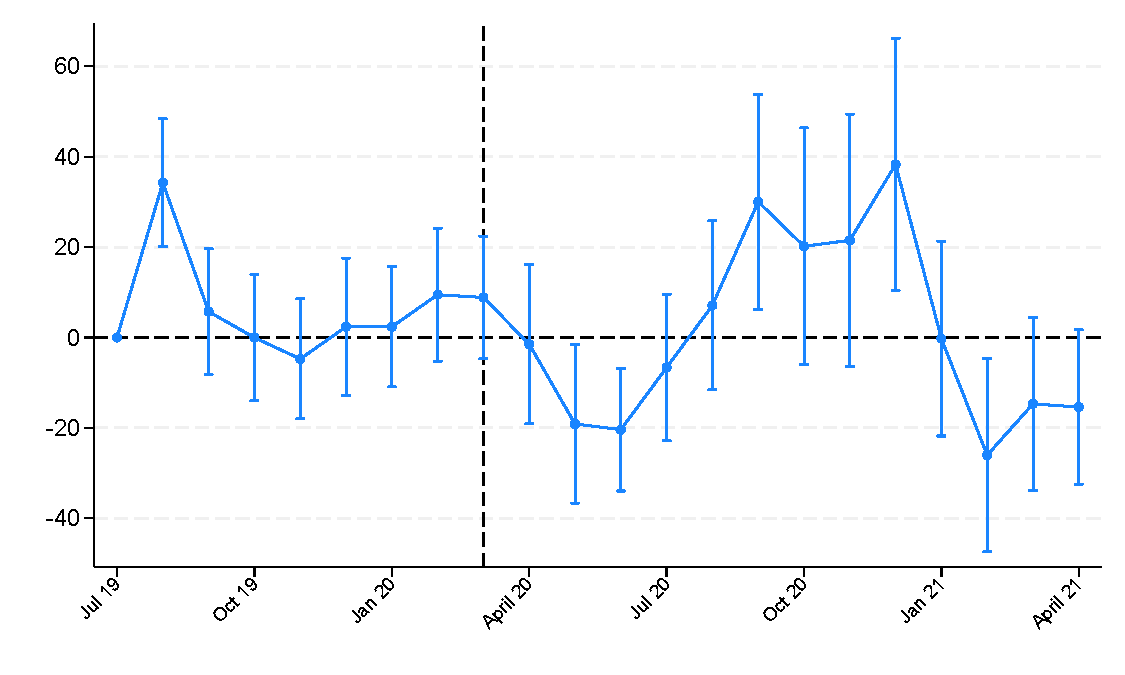
\includegraphics[width=0.998\textwidth]{../results/figures/did_loan_amount_exposure_march_dummy.pdf}
        \caption{ Loan amount }\label{fig:loan_amount}
       \end{subfigure}
       \begin{subfigure}[b]{0.49\textwidth}
        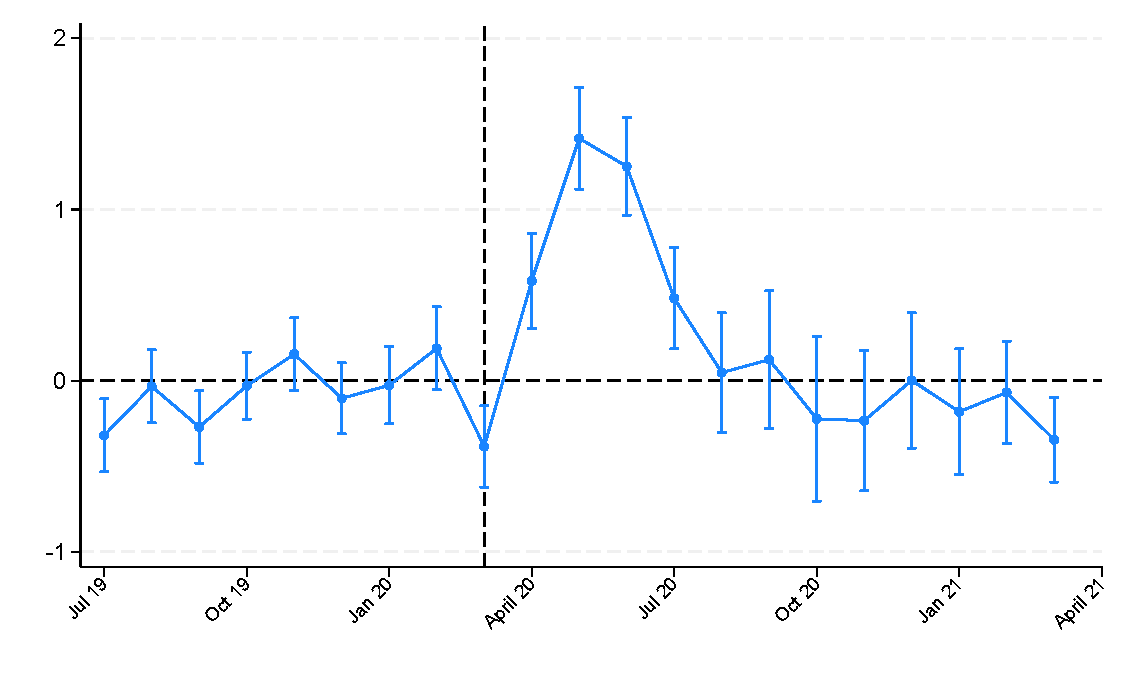
\includegraphics[width=0.998\textwidth]{../results/figures/did_winner_bid_exposure_march_dummy.pdf}
        \caption{ Winner bid }\label{fig:winner_bid}
       \end{subfigure}
       \caption{Effect of QE on Ob Auctions using exposure dummy.}\label{fig:did_exp_amount}
     \begin{minipage}{\textwidth}
        \footnotesize{\textit{Notes:} The figure shows a time series of auction outcomes for Conforming loans with a 30-year maturity. The vertical line is March 1.  } 
        \end{minipage}
  \end{figure}
  

\begin{figure}[h]
    \centering
    \begin{subfigure}[b]{0.49\textwidth}
        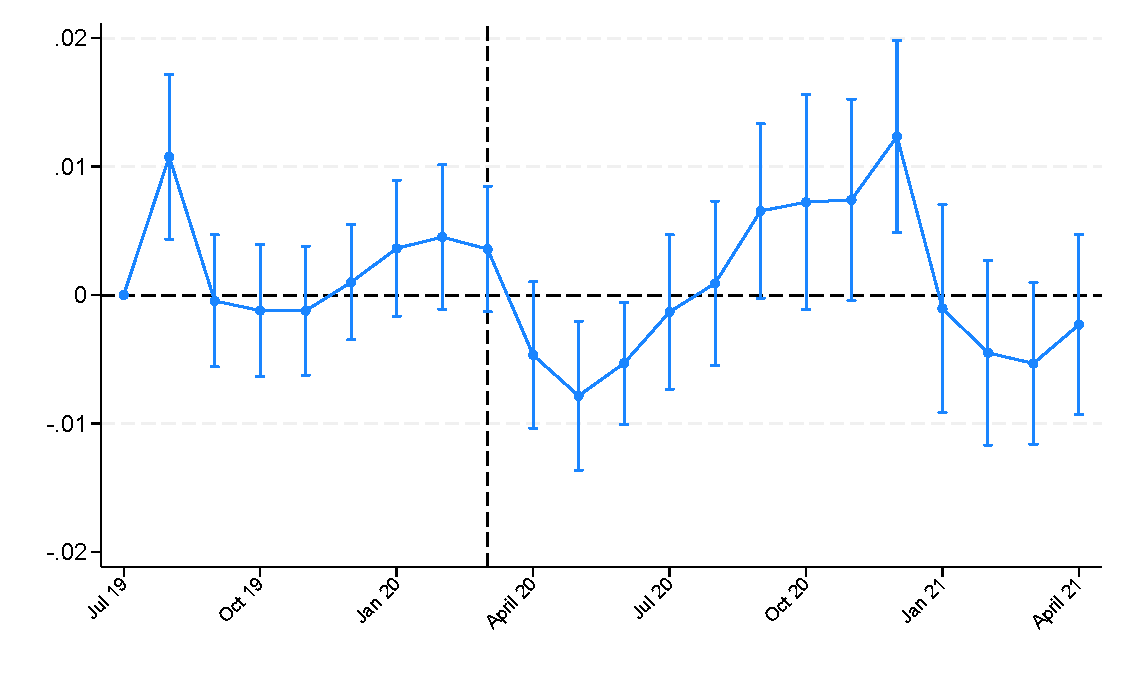
\includegraphics[width=0.998\textwidth]{../results/figures/did_loan_amount_expamount_march_dummy.pdf}
        \caption{ Loan amount }\label{fig:loan_amount}
       \end{subfigure}
       \begin{subfigure}[b]{0.49\textwidth}
        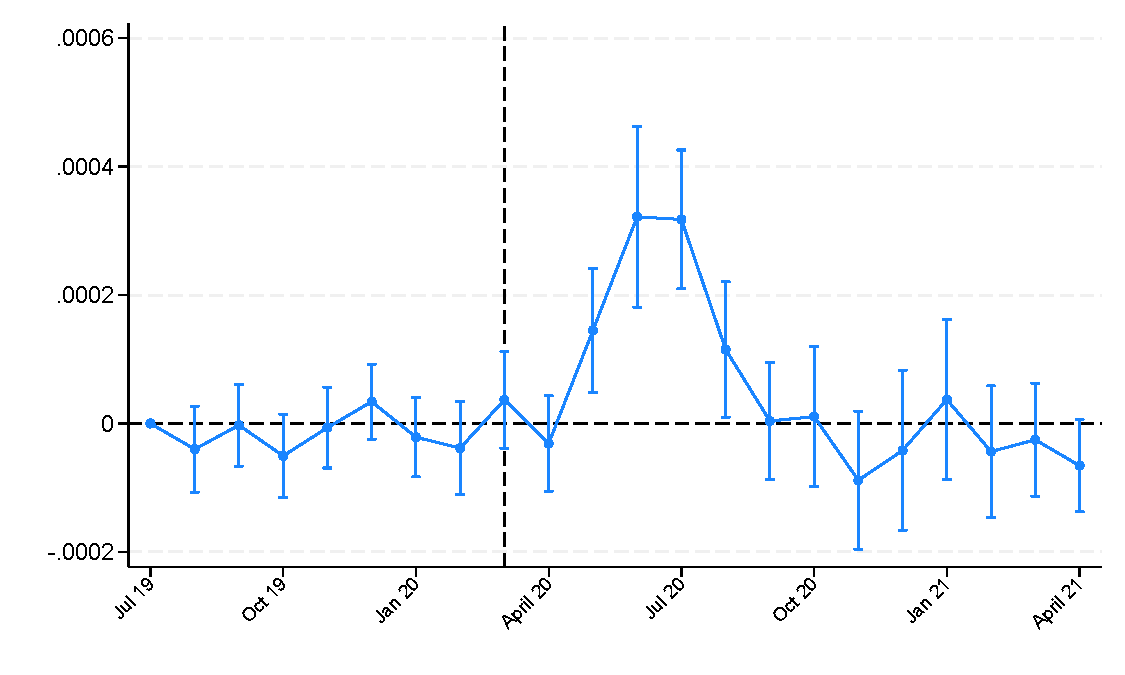
\includegraphics[width=0.998\textwidth]{../results/figures/did_winner_bid_expamount_march_dummy.pdf}
        \caption{ Winner bid }\label{fig:winner_bid}
       \end{subfigure}
       \caption{Effect of QE on Ob Auctions using exposure amount purchase.}\label{fig:did_exp_amount}
     \begin{minipage}{\textwidth}
        \footnotesize{\textit{Notes:} The figure shows a time series of auction outcomes for Conforming loans with a 30-year maturity. The vertical line is March 1.  } 
        \end{minipage}
  \end{figure}
  



\end{document}
